\section{The tool boundary}
\label{sec:boundary}

The previous two sections described the record a run keeps (\cref{sec:state}) and the code that
reads that record to choose the next node or to stop (\cref{sec:control}). This section describes
the \textbf{tool boundary}, the point at which an action the model requests becomes an action the
runtime executes, or refuses to execute. Every tool call the model makes crosses this point, so this
is where the runtime decides which requested tool actions are executed. We describe what a tool
contract specifies, how the dispatcher checks and executes a request, which records prove that a
tool ran, how the design of an agent's tools affects its performance, and which guarantees the
runtime enforces.

% Set here, ahead of the subsection that walks it, so that the figure reaches the page on which
% that subsection begins.
\begin{figure*}[t]
  \centering
  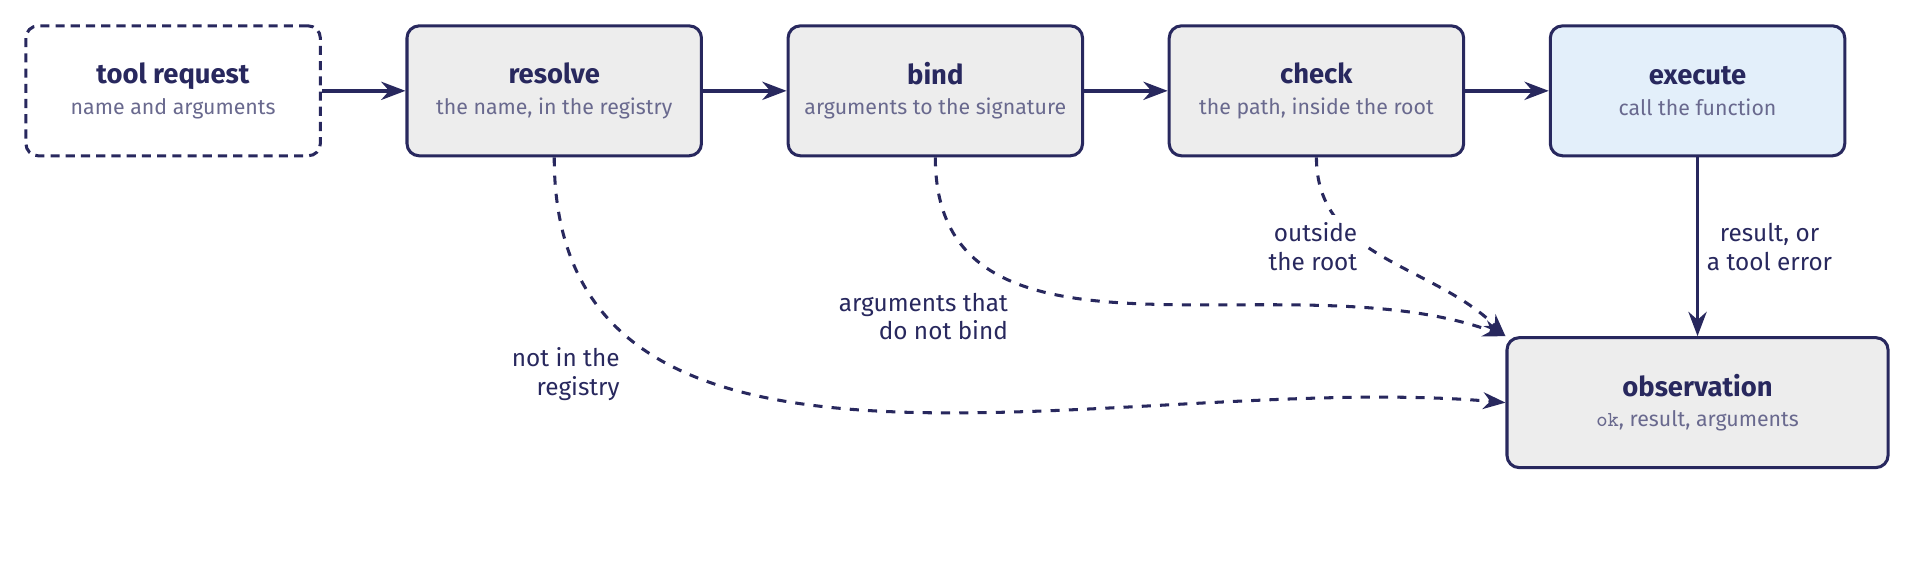
\includegraphics[width=\textwidth, trim=0 26bp 0 0, clip]{figures/deck/dispatch-cycle.png}
  \caption{One tool request through the dispatcher. Along the solid arrows, the name is found in the
  registry, the arguments bind to the function's signature, the path lies inside the workspace root,
  and the function is called. The dashed arrows are the three refusals. Every path, including a tool
  error, ends in an observation.}
  \label{fig:boundary-dispatch}
\end{figure*}

\subsection{What a tool contract contains}
\label{sec:boundary-contract}

A tool has two faces: the definition the model reads, and the implementation the runtime runs. Only
the definition reaches the model. As defined in \cref{sec:agents-msa}, a tool is an operation that the
agent requests by name, with arguments, and that the runtime carries out on its behalf. The model
never runs a tool itself. It emits a tool call, a request to run one of its tools
(\cref{sec:reactive-loop}), and the runtime decides what happens to that request.

A \textbf{tool contract} is the complete specification of one tool. It has five parts:
\bi
\item \textbf{Name and purpose.} The contract states what the tool is called and what it is for.
\item \textbf{Typed arguments.} The contract lists the arguments the tool accepts, with their types
and any constraints on their values.
\item \textbf{Result and error.} The contract gives the type of a successful result and the form in
which an error is reported.
\item \textbf{Side-effect class.} The contract says whether the tool only reads its environment or
also changes it. In our running example, \demoref{read\_file} and \demoref{search} only read, and
\demoref{edit} changes a file.
\item \textbf{Execution constraints.} The contract limits where and how the tool may operate, for
example by requiring that every file the tool touches lies inside the working tree
(\cref{sec:agents-environment}).
\ei

The two faces divide these parts between them:
\bi
\item \textbf{What the model reads.} The \textbf{tool definition} is the part of the contract that
the model receives: the tool's name, a description of its purpose, and an \textbf{argument schema},
the list of the tool's arguments with their names and types.
\item \textbf{What the runtime holds.} The result and error, the side-effect class and the execution
constraints are properties of the implementation. The model is not shown them.
\ei

A tool definition is therefore an incomplete account of the tool. A definition can say that a tool
only reads files, but only the implementation, and the runtime that dispatches it, can make that true
(\cref{sec:boundary-dispatch,sec:boundary-guarantees}).

\subsection{One request through the dispatcher}
\label{sec:boundary-dispatch}

Every tool call the model makes passes through the dispatcher, which decides whether and how to
execute it. The dispatcher is the part of the runtime that executes tool calls (\cref{sec:state-records}).
Before it executes a call, it checks the name, the arguments and any paths in the request. After the
call, it reports the outcome. In our running example, the dispatcher does the work of the
\demoref{tools} node. When the model's reply contains a tool call, the run moves to \demoref{tools}
(\cref{sec:control}), and the dispatcher handles the call there.

The dispatcher relies on two things that the runtime owns, a registry and a workspace. The
\textbf{registry} is the table that maps each tool name to the function that implements it. The
workspace is the directory that holds the run's working tree, the copy of the fixture that the run
may read and edit (\cref{sec:state-schema}). In our running example, the fixture is OWASP
BenchmarkPython at the pinned commit. The \textbf{workspace root} is the path of the workspace.

One request passes through five operations, in order (\cref{fig:boundary-dispatch}). Resolving the
name, binding the arguments and checking the path are checks, and each can stop the request. A
\textbf{refusal} is the dispatcher's decision, at one of these checks, not to call the function.
\bi
\item \textbf{Resolve the name.} The dispatcher looks the tool's name up in the registry. A request
that names a tool outside the registry is refused. The refusal lists the tools that do exist, so the
model can correct its request.
\item \textbf{Bind the arguments.} The dispatcher matches the model's arguments to the parameters of
the tool's function, its signature. A wrong argument name, or a wrong number of arguments, is refused
with a message the model can read.
\item \textbf{Check the path.} The dispatcher applies the tool's execution constraint on paths. It
resolves every path argument, that is, rewrites it as the absolute location it really names
(\cref{sec:boundary-guarantees}), and refuses a path that lies outside the workspace root. No file is
opened before this check passes.
\item \textbf{Execute.} The dispatcher calls the function. The function returns a result, or it fails
with a \textbf{tool error}, a failure inside the function itself.
\item \textbf{Observe.} The dispatcher records the outcome as an observation and writes a
\demoref{tool\_result} event to the trace.
\ei

The observation produced in the last operation is the result of one tool call as the runtime records
it (\cref{sec:reactive-loop}). It carries three things: an \demoref{ok} flag, which is true only when the
call succeeded; the result or the error; and the arguments of the call.

The trace, the log of events the runtime writes during a run, holds two events for each call
(\cref{sec:state-records}). The \demoref{tool\_request} event records the call as the dispatcher received
it, and the \demoref{tool\_result} event records its outcome.

A request can stop early at three points, which the figure draws as dashed arrows: a name that is not
in the registry, arguments that do not bind, and a path outside the workspace root. A request that
passes all three checks reaches the function, which may still fail. Every one of these paths ends in
an observation, the same kind of object that a successful call produces. Because every path produces
an observation, a run can continue after a refusal (\cref{sec:boundary-refusal}).

The registry and the binding step each have a property that the guarantees of
\cref{sec:boundary-guarantees} rely on:
\bi
\item \textbf{One list of tools.} The registry is built from the same list of tools as the tool
definitions shown to the model. No tool can therefore be offered to the model without also being
registered with the dispatcher.
\item \textbf{Binding and types.} Binding checks the names and the number of the arguments. It does
not check their types in general. When a type mismatch is unambiguous, the dispatcher converts the
value instead of refusing it. This conversion is called \textbf{coercion}. If the model passes the
string \texttt{"12"} where the function expects an integer line number, for example, the dispatcher
converts it to 12. A refusal would spend a model call only to tell the model that its string should
have been an integer.
\ei

\subsection{Why a refusal is an observation}
\label{sec:boundary-refusal}

The dispatcher reports a refusal to the model in the same form as a result, so that the run can
continue after it. A runtime has two ways to report that a tool call did not succeed, and they have
different effects on the run:
\bi
\item \textbf{An exception.} An exception that is not handled ends the run. We reserve exceptions for
conditions from which the run cannot recover, such as a trace that cannot be written.
\item \textbf{An observation.} An observation goes back to the model. The model reads what went wrong
and chooses its next action.
\ei

A tool error is handled the same way. In our running example, \demoref{edit} replaces one piece of
text in a file with another. When the text to be replaced occurs more than once in the file,
\demoref{edit} reports the target as ambiguous instead of changing the file. The model reads this
observation and retries with more of the surrounding text. If the failure were raised as an
exception instead, the run would end at its first imprecise edit.

The reactive loop of \cref{sec:reactive} depends on this choice. The loop works because the model
sees the result of each action, and an unsuccessful action is also a result that the model can act
on.

A refusal and a tool error reach the model in the same form. Both become observations whose
\demoref{ok} flag is false, and the flag is what separates them from a success. They differ in where
the request stopped. A refused request never reaches the function that implements the tool. A
request that ends in a tool error entered the function and failed inside it.

\subsection{Why configuration is not a tool parameter}
\label{sec:boundary-config}

A run's \textbf{configuration} is the set of settings we fix for it before it starts. It must never
be a parameter of a tool's function, because the model can set every parameter that the dispatcher
does not fill itself. The reason lies in how the dispatcher binds arguments. In code, the signature
of \demoref{read\_file} and the call that binds the model's arguments to it look like this
(\cref{lst:boundary-bind}):

\noindent\begin{minipage}{\linewidth}% keeps the listing in one column
\begin{lstlisting}[basicstyle=\ttfamily\scriptsize, columns=fullflexible, keepspaces=true, breaklines=false, caption={The signature of \demoref{read\_file}, and the call with which the dispatcher binds the model's arguments to it.}, label=lst:boundary-bind]
def read_file(ws: Path, path: str, start: int | None = None,
              end: int | None = None) -> str:
    ...

inspect.signature(function).bind(self.ws, **args)
\end{lstlisting}
\end{minipage}

The function \demoref{read\_file} takes four parameters: \demoref{ws}, the workspace root;
\demoref{path}, the file to read; and \demoref{start} and \demoref{end}, an optional range of lines.
The last line is the dispatcher's binding call, in which \demoref{function} is the function the
registry returned for the requested name. Python's \demoref{inspect.signature(...).bind} checks that
a set of arguments fits a function's parameters, without calling the function.

The dispatcher passes its own workspace root, \demoref{self.ws}, as the first argument. It then
matches the model's arguments, \demoref{**args}, by name to the parameters that remain. If a name
matches no parameter, or a required parameter is missing, binding fails and the dispatcher refuses
the request.

Every parameter after the workspace root is a value the model is permitted to supply. Suppose we gave
\demoref{read\_file} a \demoref{config} parameter carrying the run's configuration. Binding would
accept a \demoref{config} argument from the model like any other, so the model could set it. For
this reason our tools read the run's configuration from a module rather than accepting it as a
parameter, and no argument from the model can reach it there.

The workspace root is also a parameter, but the dispatcher supplies it. It does not appear in the
argument schema the model reads, so the model never sees it and has no way to pass it. Whether a
parameter is under the model's control therefore depends on who fills it when the dispatcher binds
the call.

\subsection{The artifacts of one tool call}
\label{sec:boundary-artifacts}

A single tool call leaves a series of artifacts, and each one establishes a different claim about
what happened. Each is an artifact in the sense of \cref{sec:fixed-definition}: something that a
later step, or a person examining the run, can read.

\Cref{tab:boundary-artifacts} follows one \demoref{read\_file} call from our running example, in
which the model reads the file that the alert flags. The rows follow the call in the order in which
each artifact arises. The last row adds a \textbf{tool message}, the message that carries a tool's
result back to the model. The rows to compare are the model response and the \demoref{tool\_result}
event, because the last column shows that they establish very different things.

\begin{table}[htbp]
  \centering
  \caption{The artifacts that one \demoref{read\_file} call leaves, in the order they arise, and the
  claim each one supports.}
  \label{tab:boundary-artifacts}
  \begin{adjustbox}{width=\linewidth}\begin{tabularx}{\linewidth}{@{}L{0.22\linewidth}L{0.36\linewidth}X@{}}
    \toprule
    \textbf{Artifact} & \textbf{What it contains} & \textbf{What it establishes} \\
    \midrule
    \textbf{Model input} & The tool definitions and the conversation so far & Which operations
      were offered, and on what description \\
    \textbf{Model response} & A tool call: an identifier, a name, arguments & That the model
      requested an operation. Nothing more \\
    \textbf{\demoref{tool\_request}} & The name and arguments as the dispatcher received them &
      That the request reached the dispatcher \\
    \textbf{Dispatcher} & Registry lookup, argument binding, path resolution & That the request
      satisfied the contract, or why it did not \\
    \textbf{\demoref{tool\_result}} & \demoref{ok=true} and the length of the result & That the
      function ran and returned \\
    \textbf{State and next input} & One observation appended, one tool message appended & What the
      next model call was allowed to see \\
    \bottomrule
  \end{tabularx}\end{adjustbox}
\end{table}

The first two artifacts belong to the conversation with the model. The tool call is kept in the
conversation's message history in the form in which the model provider, the service that hosts the
model, returned it. The trace records the same call as the dispatcher received it, in the
\demoref{tool\_request} event. The two copies come from different sources: the first is what the
model provider returned, and the second is what the runtime received and acted on.

The model response and the \demoref{tool\_result} event establish different things. The model
response shows only that the model requested an operation. The \demoref{tool\_result} event, with
\demoref{ok=true}, shows that the function ran and returned. Between the two sit the dispatcher's
checks, any one of which could have refused the request. When a check refuses the request, the
refusal is the error carried by the \demoref{tool\_result} event.

The last artifact determines what the model sees next. The observation is appended to state, and its
text is appended to the conversation as a tool message. The next model call is built from that
conversation.

% The ablation table of \cref{sec:boundary-ablation} is set here, ahead of its text, so that it can
% float to the top of a page before the References.
\begin{table*}[t]
  \centering
  \caption{Percentage of SWE-bench Lite resolved by SWE-agent and by variants of its interface, with
  the backbone model held fixed. Each variant changes one component, and Change is measured against
  the configured system.}
  \label{tab:boundary-ablation}
  \begin{adjustbox}{width=\linewidth}\begin{tabularx}{\linewidth}{@{}L{0.18\linewidth}Xrr@{}}
    \toprule
    \textbf{Component} & \textbf{Variant} & \textbf{Resolved} & \textbf{Change} \\
    \midrule
    \textbf{SWE-agent} & as configured & 18.0 & \\
    \textbf{Editor} & edit command without linting & 15.0 & $-3.0$ \\
     & no edit command (shell only) & 10.3 & $-7.7$ \\
    \textbf{Search} & iterative search & 12.0 & $-6.0$ \\
     & no search commands (shell only) & 15.7 & $-2.3$ \\
    \textbf{File viewer} & 30-line window & 14.3 & $-3.7$ \\
     & whole file & 12.7 & $-5.3$ \\
    \textbf{Context} & full history & 15.0 & $-3.0$ \\
     & no demonstration & 16.3 & $-1.7$ \\
    \bottomrule
  \end{tabularx}\end{adjustbox}
\end{table*}

\subsection{What proves a function ran}
\label{sec:boundary-evidence}

Only a record written by the runtime, the \demoref{tool\_result} event, can show that a function ran.
A model response shows only that a tool was requested. The kinds of evidence a run offers differ in
what they can show:
\bi
\item \textbf{A tool call in a model response.} This is evidence about the model: it asked for an
operation. It is not evidence about the file system, because nothing has been executed when the
model replies.
\item \textbf{Text that shows a request and a plausible result.} This establishes nothing about
execution. A model can write text that looks like a tool call followed by its result. When the model
produced both, the text shows only what the model wrote.
\item \textbf{The \demoref{tool\_result} event.} This is the runtime's own record of the dispatch,
written by the dispatcher and never by the model. With \demoref{ok=true}, it records that the
function was called and returned. With \demoref{ok=false}, the error it carries describes what went
wrong: a refusal by one of the checks, in which case the function was never called, or a tool error
inside the function.
\ei

When one model response contains several tool calls, the dispatcher handles them one at a time and
returns one observation for each, including the calls that were refused or failed. Each tool call
carries an identifier, and the next request to the model must answer every call with a tool message
that repeats its identifier. A tool call left without an answer makes that request malformed, so
every call must be answered.

\subsection{The agent-computer interface}
\label{sec:boundary-aci}

The design of an agent's tools, and of the results they return, affects how well the agent performs,
separately from the model it uses. Together, the tools and the form of their results make up an
agent-computer interface.

\begin{definition}[Agent-computer interface]
\label{def:boundary-aci}
An agent-computer interface ``specifies both the commands available to the LM and how the
environment state is communicated back to the LM''~\citep[\S2]{yang2024sweagent}.
\end{definition}

Here LM means language model. In plain words, the \textbf{agent-computer interface} is the set of
actions an agent can take on a computer, together with the form in which it receives their results.
In \msa{}, the interface is the three tools and the observations the dispatcher returns. The work on
SWE-agent, the published agent of \cref{sec:fixed-comparison}, produced four design principles for
such an interface, and each has a counterpart in our dispatcher:
\bi
\item \textbf{Simple, few actions.} The set of actions is small and each one is easy to use. \msa{}
offers three tools, \demoref{read\_file}, \demoref{search} and \demoref{edit}.
\item \textbf{Consolidated operations.} An important operation, such as navigating or editing a
file, is consolidated into as few actions as possible, so that one action makes real progress. A single \demoref{edit} call locates a piece of text in a file and
replaces it.
\item \textbf{Informative, concise feedback.} Each result tells the model what it needs to know and
little else. When the dispatcher refuses an unknown tool name, its refusal lists the tools that do
exist.
\item \textbf{Guardrails.} The interface catches the mistakes that models commonly make, so that an
error does not carry through the turns that follow. The dispatcher refuses arguments that do not bind
and paths outside the workspace root, and \demoref{edit} reports an ambiguous target instead of
changing the file.
\ei

SWE-agent's overall results suggest that the interface matters. SWE-bench is a benchmark of 2,294
issues from open-source Python repositories, and SWE-bench Lite (\cref{sec:fixed-agentless}) is a
300-issue subset of it. On SWE-bench, SWE-agent with GPT-4 Turbo resolved 12.47\% of the issues.

The previous best system resolved 3.8\%. It was a non-interactive, retrieval-augmented system: it
retrieved the files most likely to be relevant and asked the model to write a patch from them,
without taking any action in the repository.

The same interface also carried over to another model. With Claude 3 Opus, SWE-agent resolved
10.5\%.

These are comparisons between whole systems, which differ in more than their interface, so they do
not show that the interface alone caused the difference. That evidence comes from an
\textbf{ablation}, an experiment that changes or removes one component of a system at a time, keeps
everything else fixed, and measures the effect (\cref{sec:boundary-ablation}).

\subsection{What each interface component is worth}
\label{sec:boundary-ablation}

An ablation of SWE-agent's interface shows that single interface choices change how many issues the
agent resolves. In this ablation, the backbone model (\cref{sec:reactive-failures}), the language model the
agent calls, is held fixed. The measure is the percentage of the 300 issues of SWE-bench Lite that
the agent resolves \citep[Table~3]{yang2024sweagent}. The configured system's 18.0\% differs from
the 18.33\% reported for SWE-agent in \cref{sec:fixed-comparison} because the two studies ran
SWE-agent with different backbone models.

SWE-agent runs on a Linux shell, and its interface adds commands of its own for viewing, searching
and editing files. The agent can still use the shell's ordinary commands, such as \texttt{grep} and
\texttt{sed}, when a command of the interface is removed. \Cref{tab:boundary-ablation} gives the
results. Each row changes one component and leaves the others
as configured. Every value in the Change column is therefore measured against the same baseline, the
configured system's 18.0\%, and the rows are compared by reading down that column. The components
are the following:
\bi
\item \textbf{Editor.} As configured, each edit is checked by a \textbf{linter}, a program that
detects syntax errors, and an edit that introduces such an error is discarded and the agent is
asked to edit again. Without the linting, the agent resolves 15.0\%. Without the edit command, so
that the agent must edit with shell utilities such as \texttt{sed} or by rewriting whole files, it
resolves 10.3\%, a drop of 7.7 points and the largest in the table.
\item \textbf{Search.} As configured, a search returns a summary of its matches in one result, or,
when there are more than 50, no matches and a request for a narrower query. Returning the matches
one at a time (iterative search) lowers the score to 12.0\%. Removing the search commands, so that
the agent searches with ordinary shell commands such as \texttt{grep} and \texttt{find}, lowers it
only to 15.7\%.
\item \textbf{File viewer.} The agent reads a file through a window that shows a fixed number of
lines at a time, 100 as configured. A 30-line window gives 14.3\%, and showing the whole file at
once gives 12.7\%, so both do worse than the configured window.
\item \textbf{Context.} This component decides what the model's context holds besides the current
observation: the earlier turns, and a \textbf{demonstration}, an example of a solved task included in
the prompt. As configured, the last five observations are shown in full and each earlier one is
collapsed to a single line. Keeping the full history of earlier observations instead gives 15.0\%.
Removing the demonstration gives 16.3\%.
\ei

\subsection{What the ablation does and does not show}
\label{sec:boundary-ablation-limits}

The ablation table supports some readings and not others:
\bi
\item \textbf{What it supports.} Interface choices move the outcome by several points each. The
7.7-point drop from removing the edit command is larger than the gap between many published systems
on SWE-bench Lite (\cref{sec:fixed-salt}).
\item \textbf{What it does not support.} It does not rank interfaces in general. It measures one
system, with one backbone model, on a 300-issue subset of one benchmark. A variant that helps this
agent, with this model, on these issues may not help another agent.
\ei

An ablation describes the system on which it was run. HW1 calls for the same discipline: a result
measured on one system describes that system.

The search rows show that adding an interface component can leave the agent worse off than not
adding it. Iterative search scored 12.0\%, below the 15.7\% the agent reached with only the shell's
own commands for searching.
Returning the matches one at a time invites the model to work through every match in turn. Whether
an interface choice helps must therefore be measured.

\subsection{Each guarantee, and what enforces it}
\label{sec:boundary-guarantees}

Every guarantee our runtime gives is enforced by the runtime's code or by the way the fixture is set
up, and no guarantee is enforced by an instruction in a prompt. As in \cref{sec:fixed-guarantees}, a
guarantee is a property of the program we have designed, and it holds whatever the model does. The
guarantees collected here include two limits enforced away from the tool boundary, the budget on
model calls and the attempt limit (\cref{sec:control}).

\Cref{tab:boundary-guarantees} pairs each guarantee with the component that enforces it. The path
check is made by a function called \demoref{workspace.resolve}. In the second column, every entry
names code in the runtime or a property of the fixture, and none names a prompt.

\begin{table}[!htbp]
  \centering
  \caption{The guarantees of our runtime, and the component that enforces each one.}
  \label{tab:boundary-guarantees}
  \begin{adjustbox}{width=\linewidth}\begin{tabularx}{\linewidth}{@{}XL{0.42\linewidth}@{}}
    \toprule
    \textbf{Guarantee} & \textbf{Where it is enforced} \\
    \midrule
    \textbf{Only registered tools run} & The registry, consulted before anything is called \\
    \textbf{Arguments satisfy the contract} & Signature binding and coercion, before the call \\
    \textbf{No file outside the workspace is touched} & \demoref{workspace.resolve}, on every path
      argument \\
    \textbf{Inspection does not modify the fixture} & The tool implementations, and the pinned
      commit \\
    \textbf{An exhausted budget prevents another model call} & The controller's check, made before
      each model call \\
    \textbf{A back edge obeys the attempt limit} & The routing function and the attempt counter \\
    \bottomrule
  \end{tabularx}\end{adjustbox}
\end{table}

The rows group by the component that does the checking:
\bi
\item \textbf{The dispatcher.} The guarantees about registered tools, arguments and paths are the
dispatcher's checks (\cref{fig:boundary-dispatch}). The registry is consulted before any function is
called. Binding checks the names and number of the arguments, and coercion converts unambiguous type
mismatches. Together they do not check types in general, so the guarantee that arguments satisfy the
contract is narrower than its name suggests. The function \demoref{workspace.resolve} makes the path
check on every path argument.
\item \textbf{The tools and the fixture.} The tools that only inspect the code, \demoref{read\_file}
and \demoref{search}, are implemented to read and never to write. The fixture adds a second
protection. It is checked out at a pinned commit, so every run starts from the same version of the
code. A change made during one run therefore does not carry into the next.
\item \textbf{The runtime's limits.} The controller checks the budget on model calls before it issues
each model call. A back edge, an edge that leads to an earlier node of the graph (\cref{sec:reactive-graph}),
lets a rejected candidate patch start a new attempt. The routing function sends the run along it only
while the attempt counter is below the attempt limit.
\ei

A sentence in a prompt could not provide any of these guarantees. A prompt is text the model reads,
and nothing forces the model to follow it. A check in the runtime's code runs on every call, whatever
the model produces.

The path check also shows why such a check has to be written carefully. The function
\demoref{workspace.resolve} fully resolves both the workspace root and the requested path before it
compares them. To resolve a path is to rewrite it as the absolute path it really names. Every
\texttt{..}\ segment, a step up to the parent directory, is applied, and every symbolic link, a file
that points to another location, is followed. Only then does the function check that the requested
path lies inside the root.

A shortcut that compares the two paths as strings looks equivalent but is not. The root
\texttt{/tmp/ws} is a string prefix of \texttt{/tmp/ws-evil}, an unrelated directory, so a prefix
test would accept a file in \texttt{/tmp/ws-evil}. Resolving first does not repair a string
comparison, because a file in \texttt{/tmp/ws-evil} resolves to a path that still begins with the
string \texttt{/tmp/ws}. The check must ask whether the path lies inside the root directory.

\subsection{A refused request, side by side}
\label{sec:boundary-refused}

A boundary is tested most clearly by a request built to be refused, set beside one that is permitted.
Waiting for a model to produce a forbidden request is a poor test, because it may never happen, so we
construct the request ourselves. Two requests go to the same dispatcher for the same tool, and only
their arguments differ. The permitted request is an ordinary \demoref{read\_file} of a file in the
workspace. The refused request proceeds as follows:
\bi
\item \textbf{The request.} \demoref{read\_file} with the path \texttt{../../etc/passwd}, which leads
out of the workspace to a system file. We wrote this request, and the model did not make it.
\item \textbf{The check.} The path check in \demoref{workspace.resolve} raises an exception, the
dispatcher catches it, and no file is opened. The exception stays inside the dispatcher, which turns
it into an observation (\cref{sec:boundary-refusal}).
\item \textbf{The evidence.} The trace holds a \demoref{tool\_request} event and a
\demoref{tool\_result} event with \demoref{ok=false}, whose error is the path check's refusal. No
event shows that \demoref{read\_file} was called.
\ei

The two requests use the same tool and the same dispatcher and differ only in their path argument.
Because nothing else differs, the comparison shows that the argument alone decided whether the
function ran. More generally, a tool call from the model is a request: the runtime decides whether to
execute it, and it can refuse.

For any decision in a run, we can ask two questions: which component made it, and which record proves
it. For the refused request, the component is the dispatcher's path check. The records are the
\demoref{tool\_request} event and the \demoref{tool\_result} event with \demoref{ok=false}, and no
record shows that the function was called. HW1 asks the same two questions about runs on the same
fixture, with the same tools.

\subsection*{Key points}
\bi
\item The model reads only a tool's definition (its name, purpose and argument schema), and the rest
of the tool contract is a property of the implementation.
\item For each request, the dispatcher resolves the tool's name in the registry, binds the arguments,
checks every path against the workspace root, calls the function and records an observation.
\item A refusal or a tool error reaches the model as an observation rather than an exception, so the
model can read what went wrong and revise its request.
\item The model can set every tool parameter that the dispatcher does not fill itself, so a run's
configuration is never passed as a tool parameter.
\item A tool call in a model response shows only that the model asked for an operation, and only the
runtime's own record of the dispatch, the \demoref{tool\_result} event, can show that the function
ran.
\item With the backbone model held fixed, single changes to SWE-agent's agent-computer interface moved
the share of issues it resolved by several points, a result about that system rather than a ranking
of interfaces.
\item Every guarantee of the runtime is enforced by code, such as the registry, binding and the path
check, or by the fixture's pinned commit, and none by a sentence in a prompt.
\ei

% Flush this section's floats here, so that no table of this section prints after the References.
\clearpage
